\documentclass[a4paper]{article}

\usepackage[english]{babel}
\usepackage[utf8]{inputenc}
\usepackage{graphicx}
\usepackage{enumitem}
\graphicspath{ {./images/} }
    
\title{CS2200 Homework 1}
\author{Evan Wilcox}
\setlength\parindent{0pt}
    
\date{Due: January 31, 2019}
    
\begin{document}
    \maketitle

    \section{Abacus and Roman Numerals}
    \begin{enumerate}
        %1
        \item
        \begin{enumerate}
            \item X + V = XV
            \item L + I + I + I + I = LIIII = LIV
            \item C + C + X + X + X + X + V = CCXXXXV = CCXLV
            \item D + X + X + V + I + I + I = DXXVIII
            \item M + L + X + X + I + I + I + I = MLXXIIII = MLXXIV
        \end{enumerate}

        \vspace{1cm}

        %2
        \item
        \begin{enumerate}
            \item XXIV
            \begin{center}
                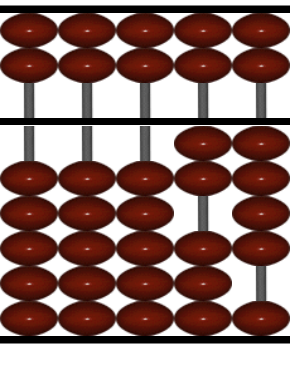
\includegraphics[scale=0.6]{2a}
            \end{center}
            
            \vspace{0.5cm}

            \item CDLV
            \begin{center}
                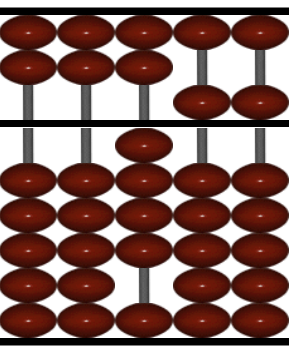
\includegraphics[scale=0.6]{2b}
            \end{center}

            \newpage

            \item CMLXXVII
            \begin{center}
                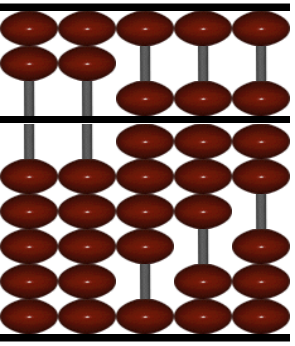
\includegraphics[scale=0.6]{2c}
            \end{center}
            
            \vspace{0.5cm}

            \item MCDL
            \begin{center}
                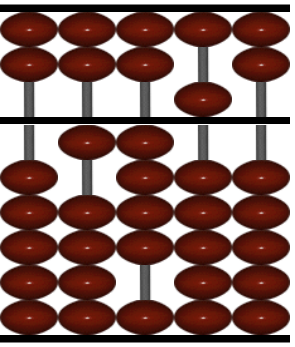
\includegraphics[scale=0.6]{2d}
            \end{center}
            
            \vspace{0.5cm}

            \item MMMDCIV
            \begin{center}
                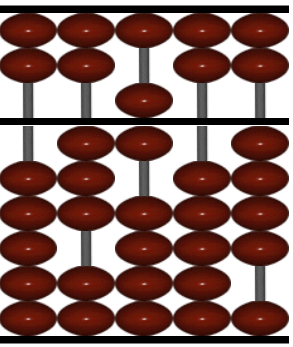
\includegraphics[scale=0.6]{2e}
            \end{center}
        
        \end{enumerate}

        \vspace{2cm}
        

        %3
        \item Here, 6 is being subtracted from 13. First subtract 10, then add 5 
              then subtract 1, i.e. 13 - 10 + 5 - 1 = 7.

        \newpage

        %4
        \item
        \begin{enumerate}
            \item Put 6 in the ones column, and then add 6 by subtracting 6's 
                  complement, 4, from the 6 in the ones column, then add a 10 in the 
                  tens column. So 6 - 4 + 10 = 12.
            
            \item Put a 10 in the tens column and 5 in the ones column, then add 9 
                  by subtracting its complement, 1, from the ones column, then add 10 
                  to the tens column. So 15 - 1 + 10 = 24.

            \item Put 3 10's in the tens column and 6 ones in the ones column, then 
                  add 75 by subtracting it's complement, 25, by removing 2 tens 
                  from the tens column and 5 ones from the ones column, then add 
                  1 100 to the 100's column. So 36 - 25 + 100 = 111.
            
            \item Put 1 10 in the ten's column, then subtract 3 by adding 3's 
                  complement, 7, to the ones column, then subtract a 10 from the 
                  10's column. So 10 + 7 - 10 = 7.
            
            \item Put 1 10 in the tens column and 2 ones in the one's column, then 
                  subtract 6 by adding it's complement, 4, to the one's column, 
                  then subtract 10 from the ten's column. So 12 + 4 - 10 = 8.
            
            \item Put 1 100 in the 100's column, then subtract 58 by adding it's 
                  complement, 42, by adding 4 10's to the ten's column and 2 1's to 
                  the one's column, then subtract 1 100 from the 100's column. 
                  So 100 + 42 - 100 = 42.
        \end{enumerate}

        %5
        \item
        \begin{enumerate}
            \item IX + VIII = VIIII + VIII = VVIIIIIII = XVII
            \item LII + CCXL = LII + CCXXXX = CCLXXXXII = CCXCII
            \item CCCXXIII + XXXV = CCCXXXXXVIII = CCCLVIII
            \item CXCV + XXI + LXXXVIII = CXXXXXXXXXV + XXI + LXXXVIII = CLXXXXXXXXXXXXXXVVIIII = CCCIV
            \item MCMXVI + MMCCCLXXXII = 
        \end{enumerate}

        %6
        \item
        \begin{enumerate}
            \item LXVIII - XII = LVI
            \item CXCII - LXIX = CLXXXVIIIIIII - LXVIIII = CXXIII
            \item XLII - XXXVIII = XXXVIIIIIII - XXXVIII = IV
            \item CCCXCV - CXV - LXX = CCCXXXXXXXXXV - CXV - XXXXXXX = CCX
            \item MMDXLVII - CMLVII = MDCCCCCCCCCLLXXXXVII - CCCCCCCCCLVII = MDLXXXX = MDXC
        \end{enumerate}

    \end{enumerate}

    \newpage

    \section{Slide Rule}

    $75.68 * 127.5 \\ = 75.68(100 + 27.5) \\ = 7,568 + 75.68(27.5) \\ = 7,568+ \sim 2,051 \\ = \sim 9,619 \\$
    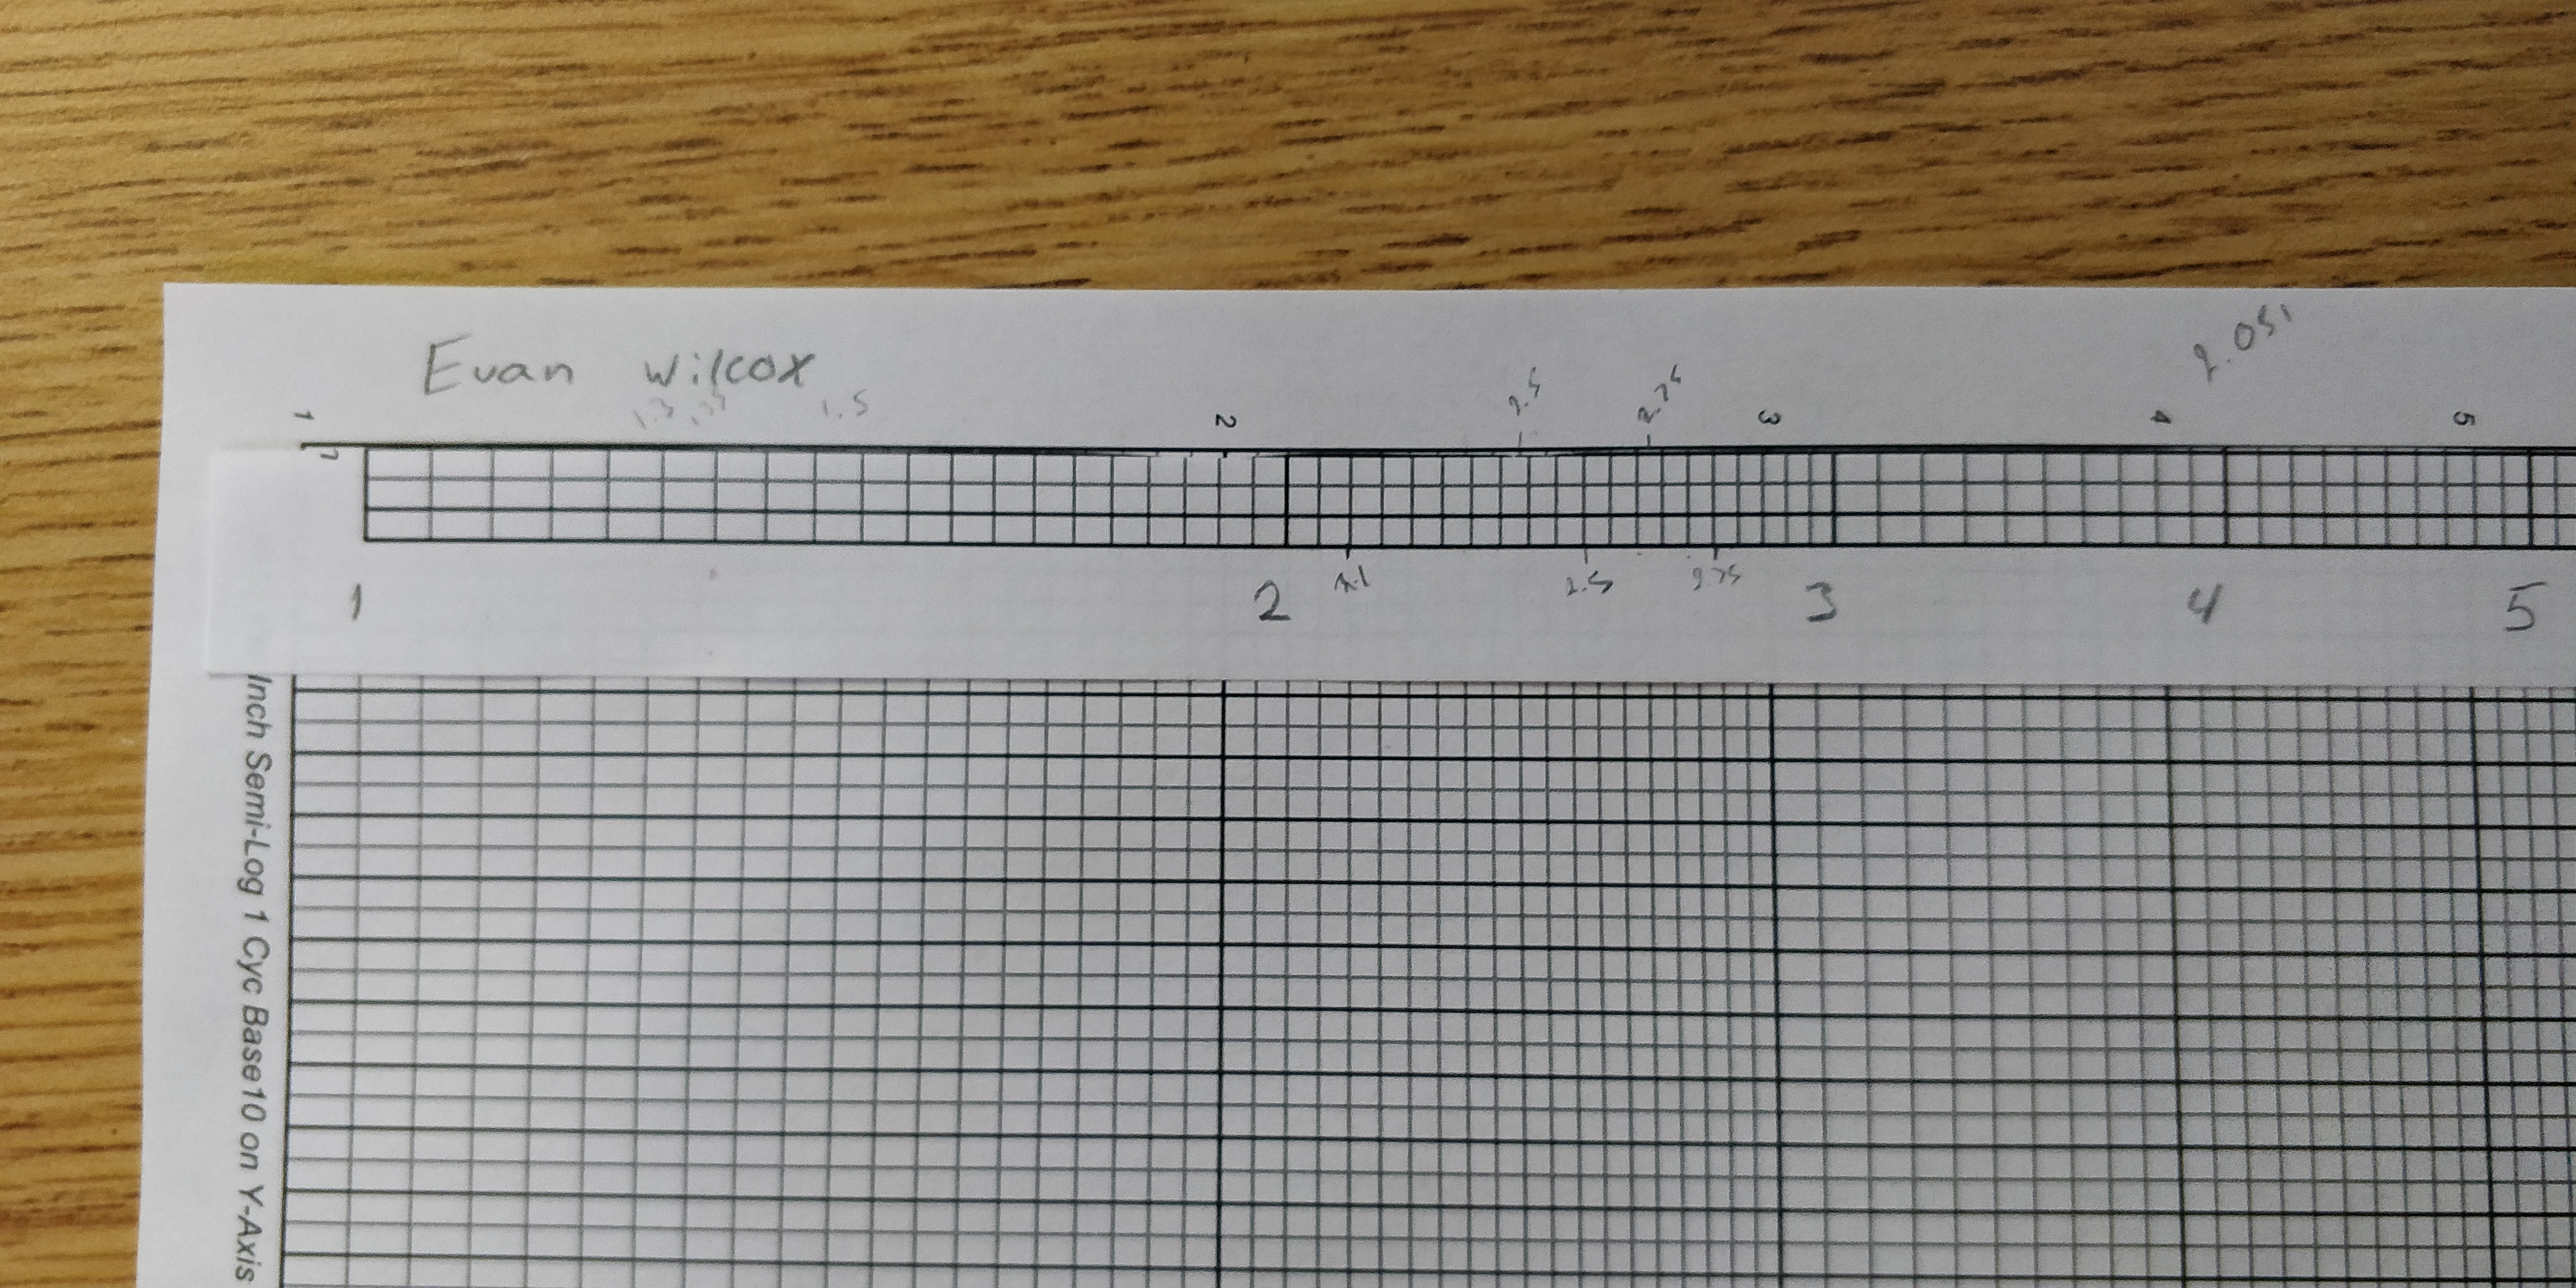
\includegraphics[scale=0.08]{2}

    \section{Napier's Bones}

    $9 * 2768 = 24,912 \\$
    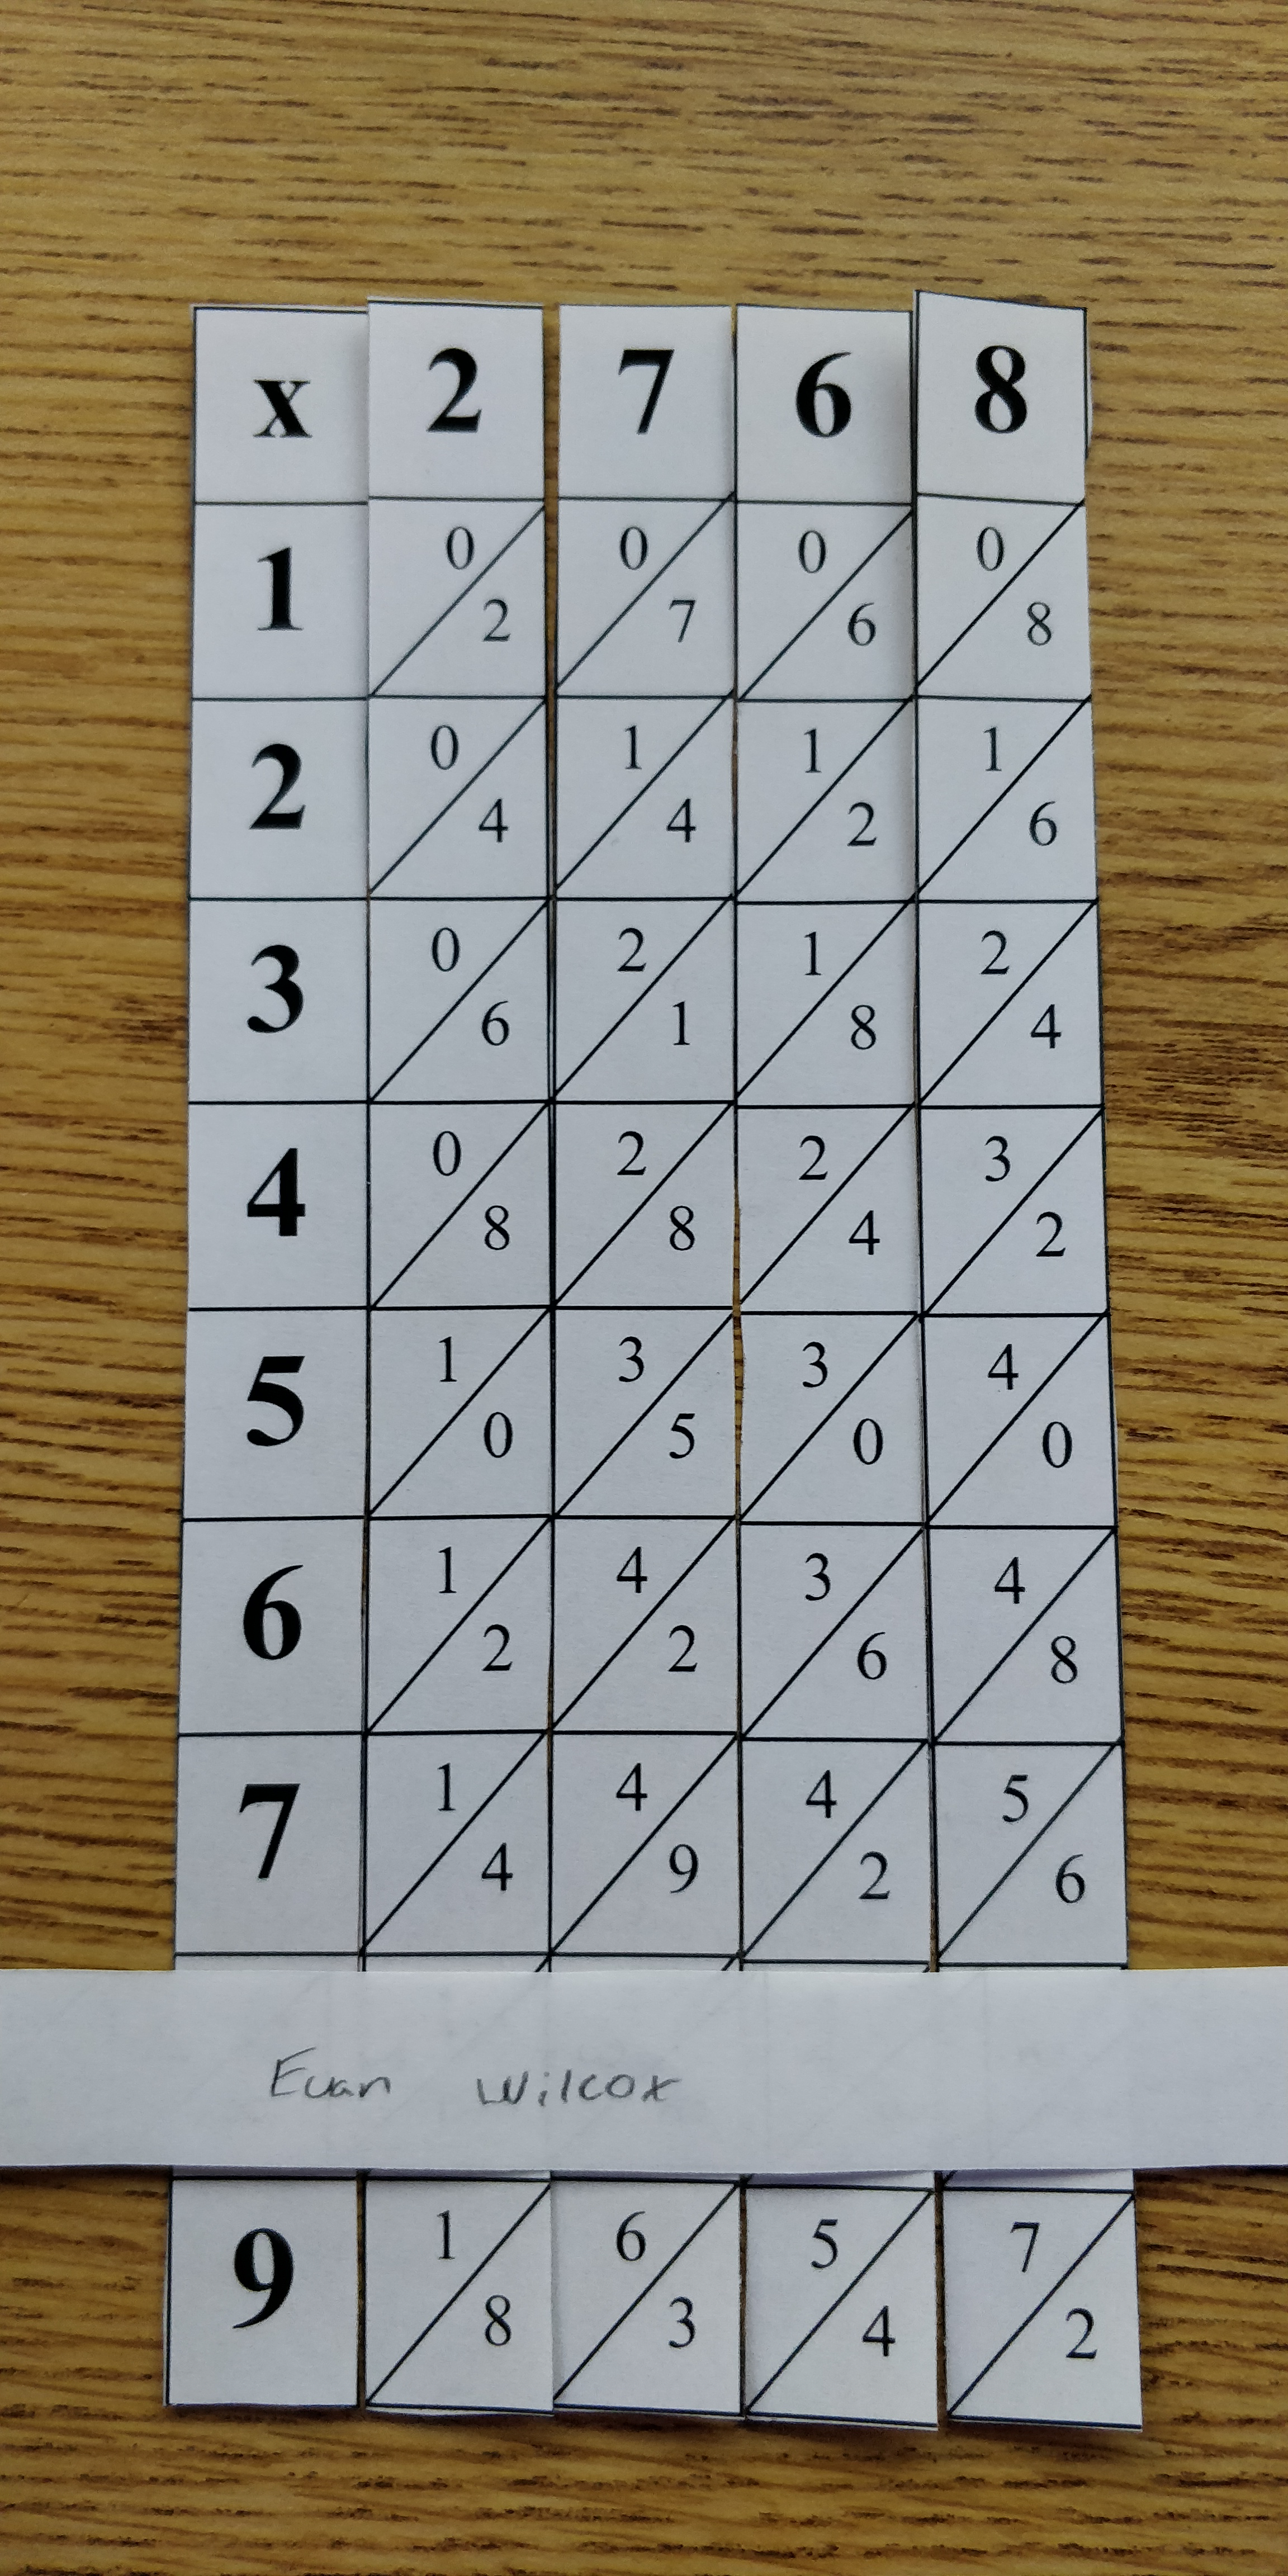
\includegraphics[scale=0.08]{3}

    \section{50 Years of Army Computing}

    \begin{enumerate}[label=\alph*)]
        \item They had to physically program the computer to do what they wanted it 
              to do by using plugboards and function tables.
        \item 20 words of read/write memory.
        \item They weren't used. There wasn't enough extra space in memory.
        \item Ballistic Research Laboratory.
        \item The IBM cards would swell with moisture because of excess humidity.
    \end{enumerate}

    \newpage

    \section{Fibonacci Representation}

    \begin{enumerate}[label=\alph*)]
        \item
        \textbf{Introduction}
        

        \textbf{Stopping Value and Two More}


        \textbf{Inductive Case}

        
        \textbf{Conclusion}

                
        \item If the string '11' was in the representation and not at the end it would imply that 
        they would combine and put a '1' in the next column and replace the '11' with '00'.



    \end{enumerate}

    \section{Fibonacci Representation Cont'd.}

    \begin{enumerate}[label=\alph*)]
    
        \item When representing a Fibonacci number using the Fibonacci representation, the number will 
        be a series of '0's followed by '11', e.g. '0000011'=13. All numbers until the next Fibonacci
        number can be representation by systematically changing the '0's to '1's.

    
        \item It seems that the number of digits in the Fibonacci representation of a number as a
        function of n is equal to $\log_\phi n + 2$ when $\phi = \frac{1+\sqrt{5}}{2}$. \\
        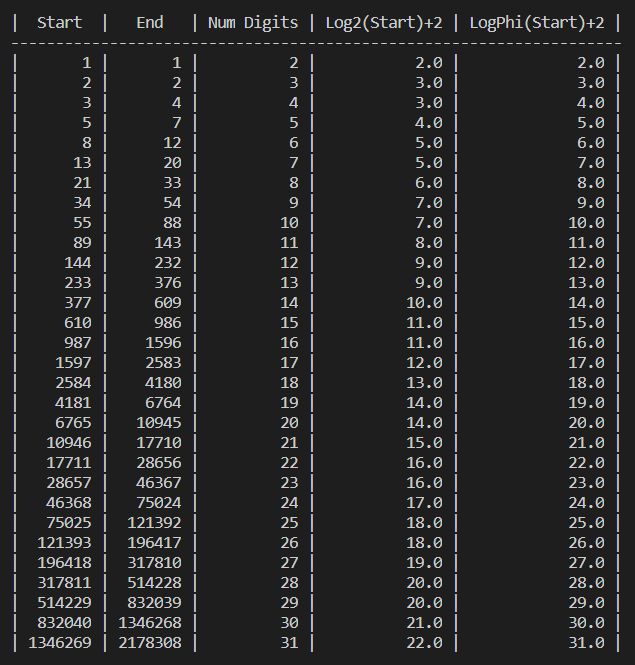
\includegraphics[scale=0.7]{6b2}\\
        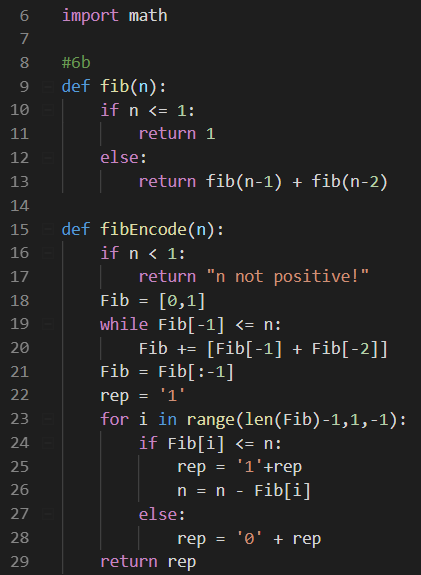
\includegraphics[scale=0.7]{6b0}\\
        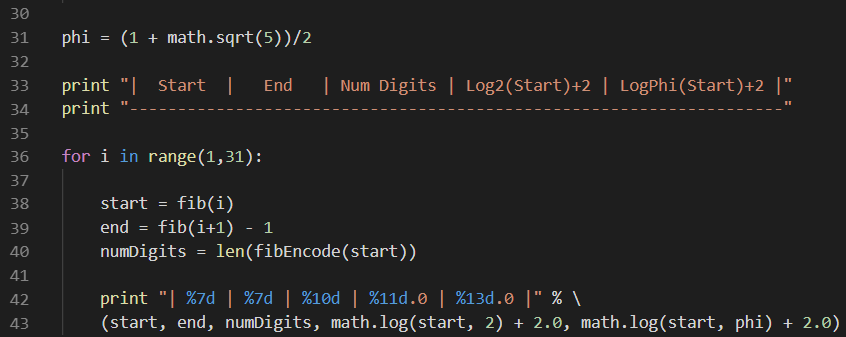
\includegraphics[scale=0.7]{6b1}
        
    
    \end{enumerate}

\end{document}